\documentclass{scrartcl}  % scrartcl of scrreprt
\usepackage{SIunits}
% Include all project wide packages here.
\usepackage{fullpage}
\usepackage{polyglossia}
\setmainlanguage{dutch}
\usepackage{csquotes}
\usepackage{graphicx}
\usepackage{epstopdf}
\usepackage{pdfpages}
\usepackage{caption}
\usepackage[list=true]{subcaption}
\usepackage{float}
%\usepackage{mathtools}
\usepackage{standalone}
\usepackage{import}
\usepackage{tocloft}
\usepackage{wrapfig}
\usepackage{authblk}
\usepackage{array}
\usepackage{booktabs}
\usepackage[toc,page,title,titletoc]{appendix}
\usepackage{xunicode}
\usepackage{amsmath}
\usepackage{fontspec}
\usepackage{unicode-math}
\usepackage[
    backend=bibtexu,
	texencoding=utf8,
bibencoding=utf8,
    style=ieee,
    sortlocale=nl_NL,
    language=auto
]{biblatex}
\usepackage{listings}
\newcommand{\includecode}[3][c]{\lstinputlisting[caption=#2, escapechar=, style=#1]{#3}}
\newcommand{\superscript}[1]{\ensuremath{^{\textrm{#1}}}}
\newcommand{\subscript}[1]{\ensuremath{_{\textrm{#1}}}}


\newcommand{\chapternumber}{\thechapter}
\renewcommand{\appendixname}{Bijlage}
\renewcommand{\appendixtocname}{Bijlagen}
\renewcommand{\appendixpagename}{Bijlagen}

\usepackage[hidelinks]{hyperref} %<--------ALTIJD ALS LAATSTE
  
\renewcommand{\familydefault}{\sfdefault}

\setmainfont[Ligatures=TeX]{Myriad Pro}
\setmathfont{Asana Math}
\setmonofont{Lucida Console}

\usepackage{titlesec, blindtext, color}
\definecolor{gray75}{gray}{0.75}
\newcommand{\hsp}{\hspace{20pt}}
\titleformat{\chapter}[hang]{\Huge\bfseries}{\chapternumber\hsp\textcolor{gray75}{|}\hsp}{0pt}{\Huge\bfseries}
\renewcommand{\familydefault}{\sfdefault}
\renewcommand{\arraystretch}{1.2}
\setlength\parindent{0pt}

%For code listings
\definecolor{black}{rgb}{0,0,0}
\definecolor{browntags}{rgb}{0.65,0.1,0.1}
\definecolor{bluestrings}{rgb}{0,0,1}
\definecolor{graycomments}{rgb}{0.4,0.4,0.4}
\definecolor{redkeywords}{rgb}{1,0,0}
\definecolor{bluekeywords}{rgb}{0.13,0.13,0.8}
\definecolor{greencomments}{rgb}{0,0.5,0}
\definecolor{redstrings}{rgb}{0.9,0,0}
\definecolor{purpleidentifiers}{rgb}{0.01,0,0.01}


\lstdefinestyle{csharp}{
language=[Sharp]C,
showspaces=false,
showtabs=false,
breaklines=true,
showstringspaces=false,
breakatwhitespace=true,
escapeinside={(*@}{@*)},
columns=fullflexible,
commentstyle=\color{greencomments},
keywordstyle=\color{bluekeywords}\bfseries,
stringstyle=\color{redstrings},
identifierstyle=\color{purpleidentifiers},
basicstyle=\ttfamily\small}

\lstdefinestyle{c}{
language=C,
showspaces=false,
showtabs=false,
breaklines=true,
showstringspaces=false,
breakatwhitespace=true,
escapeinside={(*@}{@*)},
columns=fullflexible,
commentstyle=\color{greencomments},
keywordstyle=\color{bluekeywords}\bfseries,
stringstyle=\color{bluestrings},
identifierstyle=\color{purpleidentifiers}
}

\lstdefinestyle{vhdl}{
language=VHDL,
showspaces=false,
showtabs=false,
breaklines=true,
showstringspaces=false,
breakatwhitespace=true,
escapeinside={(*@}{@*)},
columns=fullflexible,
commentstyle=\color{greencomments},
keywordstyle=\color{bluekeywords}\bfseries,
stringstyle=\color{redstrings},
identifierstyle=\color{purpleidentifiers}
}

\lstdefinestyle{xaml}{
language=XML,
showspaces=false,
showtabs=false,
breaklines=true,
showstringspaces=false,
breakatwhitespace=true,
escapeinside={(*@}{@*)},
columns=fullflexible,
commentstyle=\color{greencomments},
keywordstyle=\color{redkeywords},
stringstyle=\color{bluestrings},
tagstyle=\color{browntags},
morestring=[b]",
  morecomment=[s]{<?}{?>},
  morekeywords={xmlns,version,typex:AsyncRecords,x:Arguments,x:Boolean,x:Byte,x:Char,x:Class,x:ClassAttributes,x:ClassModifier,x:Code,x:ConnectionId,x:Decimal,x:Double,x:FactoryMethod,x:FieldModifier,x:Int16,x:Int32,x:Int64,x:Key,x:Members,x:Name,x:Object,x:Property,x:Shared,x:Single,x:String,x:Subclass,x:SynchronousMode,x:TimeSpan,x:TypeArguments,x:Uid,x:Uri,x:XData,Grid.Column,Grid.ColumnSpan,Click,ClipToBounds,Content,DropDownOpened,FontSize,Foreground,Header,Height,HorizontalAlignment,HorizontalContentAlignment,IsCancel,IsDefault,IsEnabled,IsSelected,Margin,MinHeight,MinWidth,Padding,SnapsToDevicePixels,Target,TextWrapping,Title,VerticalAlignment,VerticalContentAlignment,Width,WindowStartupLocation,Binding,Mode,OneWay,xmlns:x}
}

%defaults
\lstset{
basicstyle=\ttfamily\small,
extendedchars=false,
numbers=left,
numberstyle=\ttfamily\tiny,
stepnumber=1,
tabsize=4,
numbersep=5pt
}
\addbibresource{../../library/bibliography.bib}

\author{Erwin {de Haan} (4222814)  \\{Robin Hes} (4236815)}
\title{EPO3-1 Opdracht 5: Schmitt Trigger}
\subtitle{EE2821}
\date{14 oktober 2013}

\begin{document}
\pagenumbering{roman}
\maketitle
\vspace{80 mm}

\section*{Abstract}
\label{sec:trig-abstr}
We hebben een CMOS Schmitt Trigger geanalyseerd en gesimuleerd voor de SoG techniek en de analyse en simulatie met elkaar vergeleken.

\newpage
\setlength{\cftbeforetoctitleskip}{-3em}
\tableofcontents

\section{Inleiding}
\label{sec:trig-inl}

%TODO dit gaan we doen blaat, dat gaan we doen blaat, dit doen we hier blaat, dat doen we daar blaat

\newpage
\pagenumbering{arabic}

\section{Probleemstelling}
\label{sec:trig-prob}
De probleemstelling is zoals gegeven in opdracht 5: \\
\textit{
``Figuur 42 (uitlezen toetsenbord) uit de EPO-3 handleiding laat een Schmitt-trigger zien. Deze is gelijk
aan die uit Problem 7.7 (figuur 7-49) van het boek van Rabaey. Los dit ‘Problem’ op, maar voor SoG
transistoren met parameters uit Tabel 3 van de EPO-3 handleiding en neem voor $V_{DSAT}$ een waarde van
2V (dit is een benadering). Neem voor alle transistoren de standaard afmetingen uit het SoG image.
Vergelijk je uitkomst met simulaties en reflecteer op de overeenkomsten en verschillen.''
}
\cite[2]{epo3-opdracht-5}
\\

Problem 7.7 uit het boek van Rabaey is als volgt: \\
\textit{
``Another CMOS Schmitt trigger is shown in Figure 7-49. Discuss the operation of the gate, and derive expressions for $V_{M-}$ and $V_{M+}$.''
}
\cite[367]{rabaey-integrated-circuits}
\\

En Figure 7-49 (``Alternate CMOS Schmitt trigger'') weergeeft onderstaande schakeling:
\begin{figure}[H]
\centering
	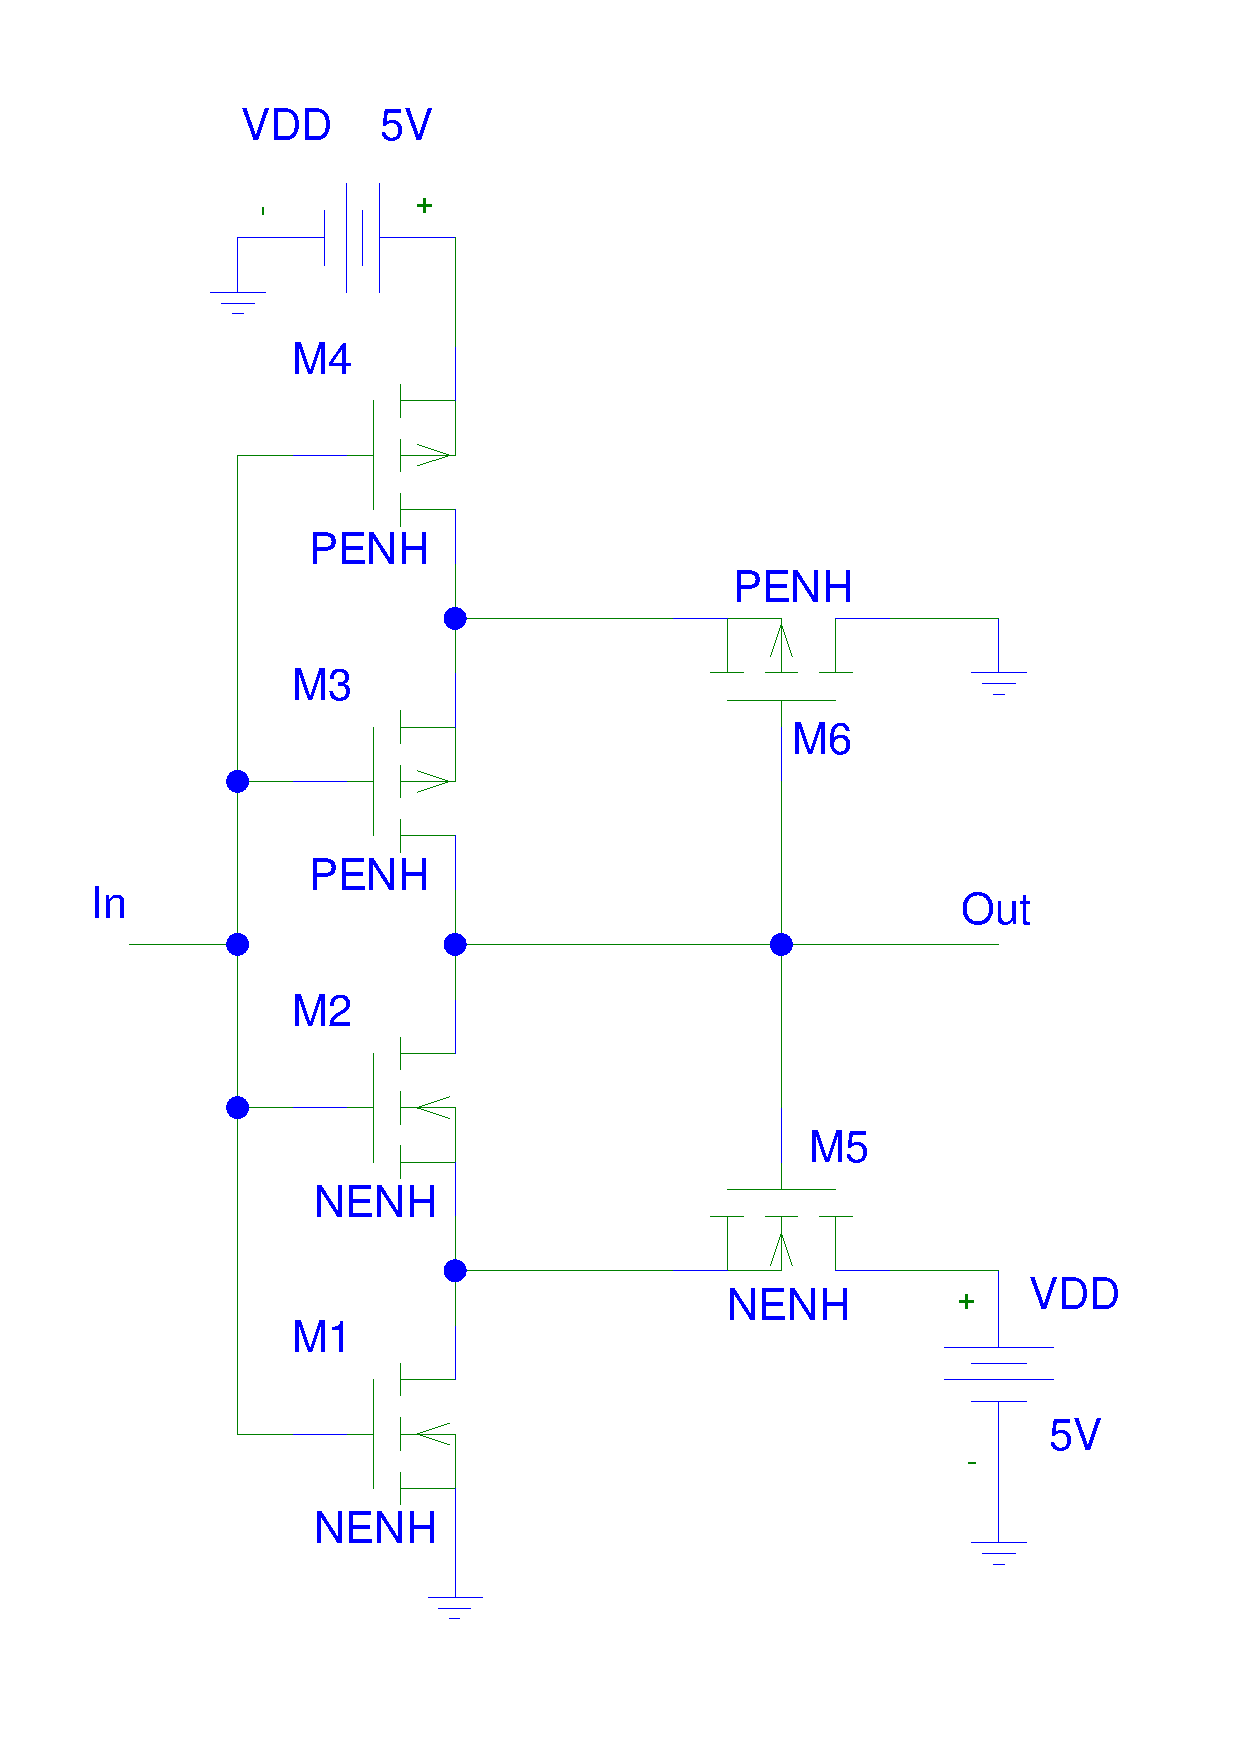
\includegraphics[width=0.6\textwidth]{resource/schmitt-rc.pdf}
	\caption{De voor deze opdracht gebruikte CMOS Schmitt trigger}
	\label{fig:schmitt-schem}
\end{figure}

\section{Theorie}
\label{sec:trig-theorie}

%TODO Schmitt trigger blaat, nonbistable blaat, blaat blaat

\section{Methode}
\label{sec:trig-methode}
$V_{M-}$ en $V_{M+}$ zijn gedefinieerd als de spanningen op knooppunt $X$ ($V_{X}$), waarvoor geldt dat de ingangsspanning van de Schmitt trigger ($V_{in}$) gelijk is aan de spanning op het knooppunt ($V_{X} = V_{in}$). Het knooppunt $X$ is het knooppunt tussen de transistoren $M_{1}$, $M_{2}$ en $M_{5}$. $V_{M-}$ en $V_{M+}$ geven een indicatie voor de schakelmomenten van de Schmitt trigger.

\subsection{M-}
\label{subsec:trig-methode-mminus}
Bij een uitgangsovergang van een logische 1 naar een logische 0 (high-to-low) is transistor $M_{6}$ in eerste instantie uitgeschakeld. Hierdoor kan de gegeven schakeling gereduceerd worden tot die in figuur~\ref{fig:schmitt-schem-high-to-low}:

\begin{figure}[H]
\centering
	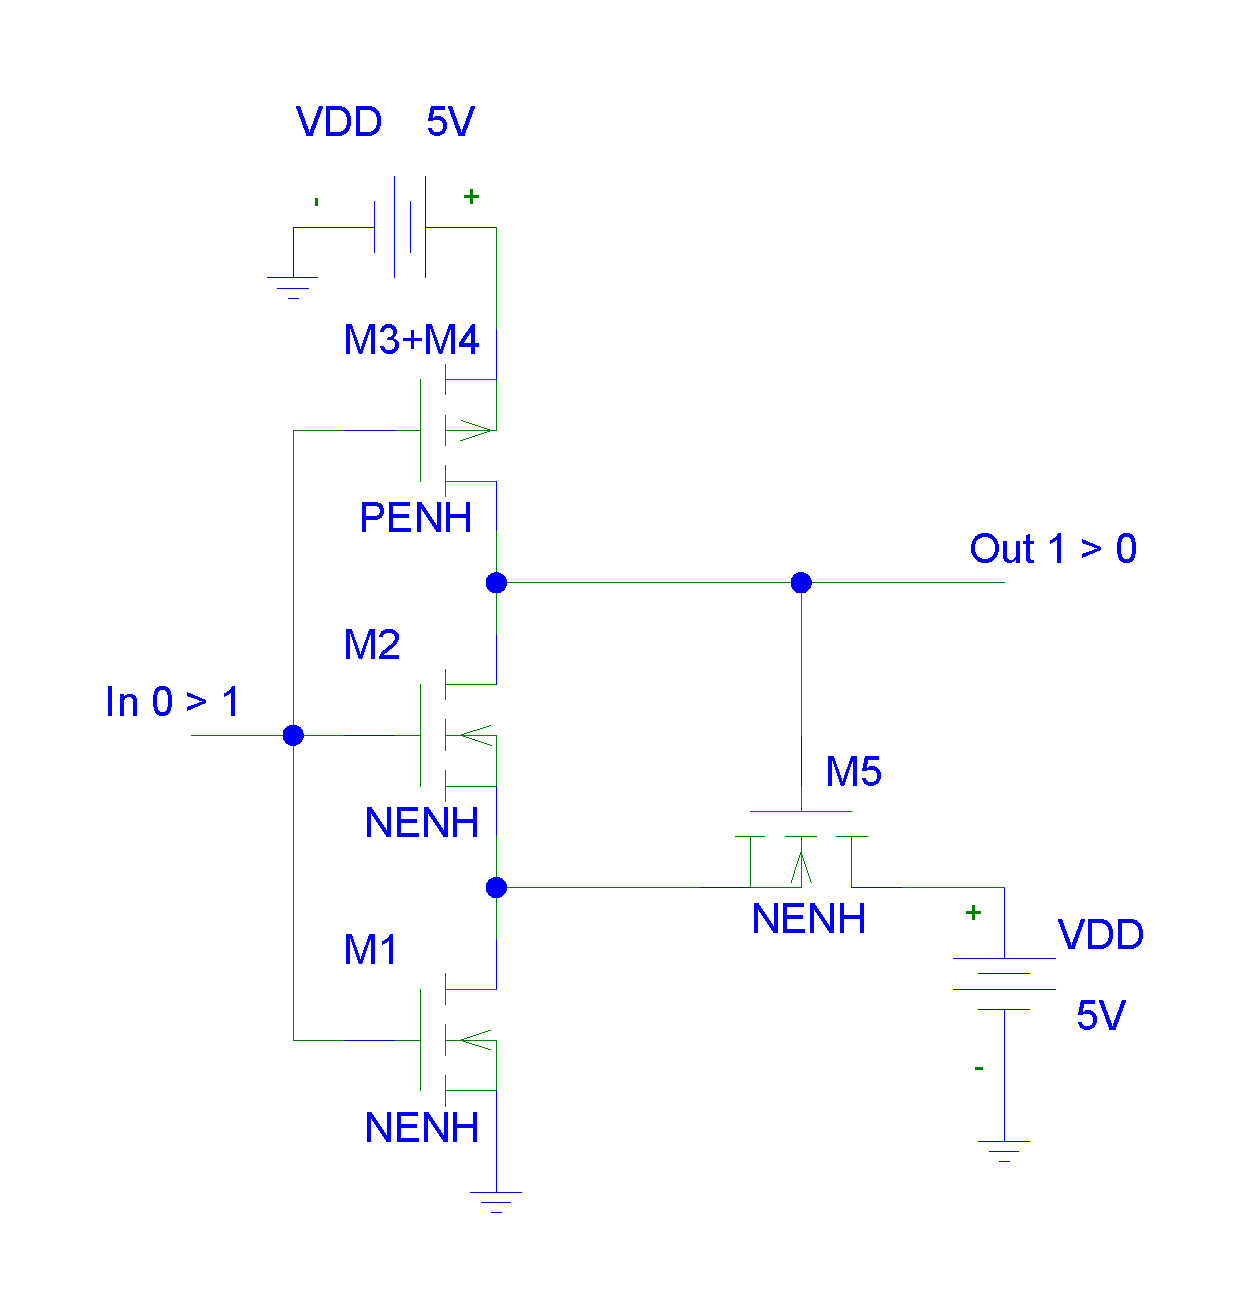
\includegraphics[width=0.6\textwidth]{resource/schmitt-high-to-low-rc.pdf}
	\caption{De vereenvoudigde schakeling voor een \textit{high-to-low}-overgang}
	\label{fig:schmitt-schem-high-to-low}
\end{figure}

Een voorwaarde voor het omslaan van de uitgang is dat de transistoren $M_{1}$ en $M_{2}$ beide aan staan. Hierdoor ontstaat een pad naar ground, waardoor $Out$ laag wordt. Transistor $M_{2}$ gaat echter pas aan, wanneer de spanning op knooppunt $X$ gestegen is tot een waarde $V_{X} = V_{in} - V_{Tn}$. Op dat punt geldt immers dat de gate-sourcespanning van $M_{2}$ groter is dan dan zijn drempelspanning ($V_{gs} = V_{in} - V_{X} > V_{Tn}$). De waarde van $V_{in}$ op dat moment (het schakelpunt) kan gebruikt worden als approximatie voor $V_{M-}$. Wanneer het body-effect verwaarloosd wordt en aangenomen wordt dat $M_{1}$ en $M_{5}$ beide gesatureerd zijn, kunnen de drainstromen door deze transistoren aan elkaar gelijkgesteld worden ($I_{D1} = I_{D5})$). Daaruit volgt onderstaande vergelijking uit het model van Rabaey:

$$k'_{n}(\frac{W}{L})_{1}((V_{M-}-V_{Tn})V_{DSATn} - \frac{V^{2}_{DSATn}}{2}) = k'_{n}(\frac{W}{L})_{5}((V_{DD}-(V_{M-}-V_{Tn})-V_{Tn})V_{DSATn} - \frac{V^{2}_{DSATn}}{2})$$

Omdat beide transistoren fysiek aan elkaar gelijk zijn geldt:

$$(V_{M-}-V_{Tn})V_{DSATn} - \frac{V^{2}_{DSATn}}{2} = (V_{DD}-V_{M-})V_{DSATn} - \frac{V^{2}_{DSATn}}{2}$$

Hieruit kan de vergelijking voor $V_{M-}$ worden afgeleid:

\begin{equation} \label{eq:schmitt-mminus}
V_{M-} = \frac{V_{DD}+V_{Tn}}{2}
\end{equation}

\subsection{M+}
\label{subsec:trig-methode-mplus}
``De andere kant op'', bij een overgang van laag naar hoog aan de uitgang (low-to-high), kan eenzelfde principe toegepast worden. Ditmaal is de spanning op knooppunt $Y$ ($V_{Y}$, het knooppunt tussen transistoren $M_{3}$, $M_{4}$ en $M_{6}$ relevant. Dit levert wederom een gereduceerde schakeling op, zoals in figuur~\ref{fig:schmitt-schem-low-to-high}:

\begin{figure}[H]
\centering
	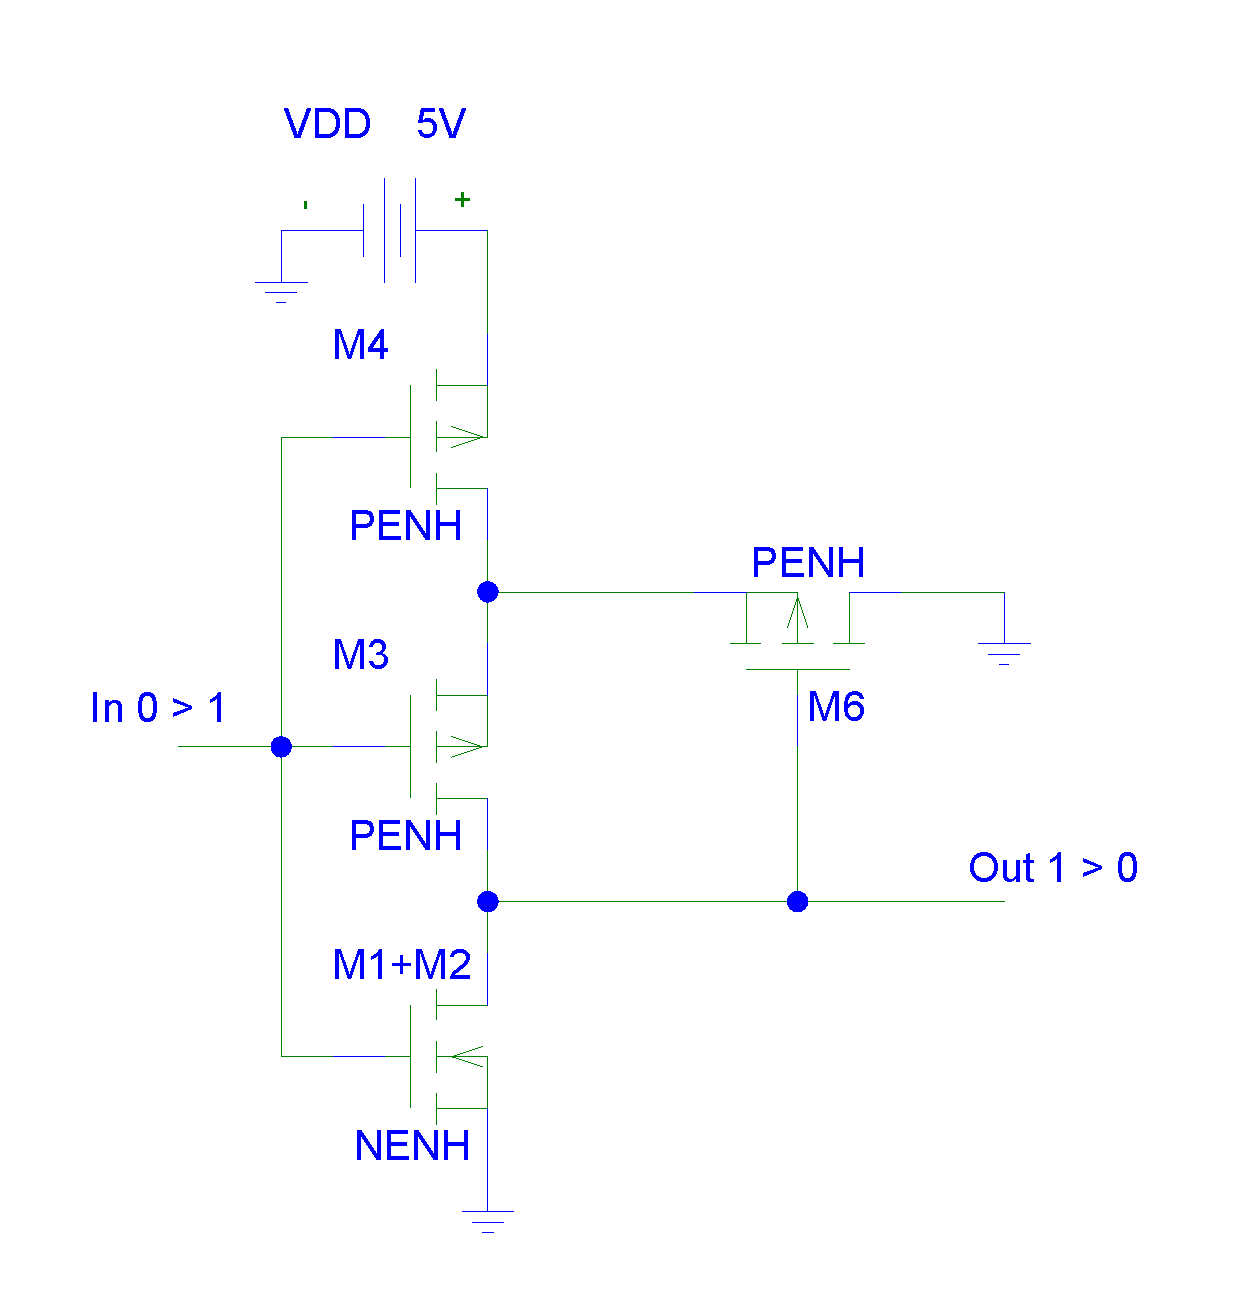
\includegraphics[width=0.6\textwidth]{resource/schmitt-low-to-high-rc.pdf}
	\caption{De vereenvoudigde schakeling voor een \textit{low-to-high}-overgang}
	\label{fig:schmitt-schem-low-to-high}
\end{figure}

Nu geldt dat het schakelmoment plaatsvindt wanneer $M_{3}$ en $M_{4}$ beide ingeschakeld zijn. $M_{3}$ gaat hierbij aan wanneer $V_{Y}$ gedaald is tot een waarde $V_{Y} = V_{in} - V_{Tp}$, omdat dan geldt dat $V_{gs} = V_{in} - V_{Y} < V_{Tp}$. Op eenzelfde manier als bij de afleiding van $V_{M-}$ kan zo de volgende vergelijking worden opgesteld voor transistoren $M_{4}$ en $M_{6}$:

$$k'_{n}(\frac{W}{L})_{4}((V_{M+}-V_{DD}-V_{Tp})V_{DSATp} - \frac{V^{2}_{DSATp}}{2}) = k'_{n}(\frac{W}{L})_{6}(-(V_{M+}-V_{Tp})-V_{Tp})V_{DSATp} - \frac{V^{2}_{DSATp}}{2})$$

Ook hier zijn de transistoren $M_{4}$ en $M_{6}$ fysiek equivalent:

$$(V_{M+}-V_{DD}-V_{Tp})V_{DSATp} - \frac{V^{2}_{DSATp}}{2} = -V_{M+}V_{DSATp} - \frac{V^{2}_{DSATp}}{2}$$

Hieruit kan de vergelijking voor $V_{M+}$ worden afgeleid:

\begin{equation} \label{eq:schmitt-mplus}
V_{M+} = \frac{V_{DD}+V_{Tp}}{2}
\end{equation}

\section{Resultaten}
\label{sec:trig-res}
\subsection{M-}
\label{subsec:trig-res-mminus}
Invullen van reeds gegeven waarden ($V_{DD} = 5 \,\textrm{V}$ en $V_{Tn} = 0.7 \,\textrm{V}$) in vergelijking~\ref{eq:schmitt-mminus} levert:

\begin{equation} \label{eq:schmitt-mminus-val}
V_{M-} = \frac{5+0.7}{2} = 2.85 \,\textrm{V}
\end{equation}

\subsection{M+}
\label{subsec:trig-res-mplus}
Invullen van reeds gegeven waarden ($V_{DD} = 5 \,\textrm{V}$ en $V_{Tp} = -1.2 \,\textrm{V}$) in vergelijking~\ref{eq:schmitt-mplus} levert:

\begin{equation} \label{eq:schmitt-mplus-val}
V_{M+} = \frac{5-1.2}{2} = 1.9 \,\textrm{V}
\end{equation}

\subsection{Simulatie en vergelijking}
\label{subsec:trig-res-verg}

%TODO er klopt geen aars van onze berekening blaat, daarom blaat

$V_{M+} = 2.500 \volt$\\
$V_{M-} = 1.566 \volt$
\begin{figure}[H]
\centering
	\setlength\figureheight{0.6\textwidth} 
	\setlength\figurewidth{0.9\textwidth}
	% This file was created by matlab2tikz v0.4.2.
% Copyright (c) 2008--2013, Nico Schlömer <nico.schloemer@gmail.com>
% All rights reserved.
% 
% The latest updates can be retrieved from
%   http://www.mathworks.com/matlabcentral/fileexchange/22022-matlab2tikz
% where you can also make suggestions and rate matlab2tikz.
% 
% 
% 
\begin{tikzpicture}

\begin{axis}[%
width=\figurewidth,
height=\figureheight,
scale only axis,
xmin=0,
xmax=5,
xlabel={$V_{IN} (V)$},
ymin=0,
ymax=4.5,
ylabel={$V_{X} (V)$},
legend style={at={(0.7,0.8)},anchor=south west,draw=black,fill=white,legend cell align=left}
]
\addplot[color=black,
solid,
line width=1.0pt] (0,0) -- (500,500);
\addlegendentry{$V_{X}=V_{IN}$};

\addplot [
color=blue,
solid,
line width=1.0pt
]
table[row sep=crcr]{
0 4.406898021698\\
0.01 4.40689849853516\\
0.02 4.40689849853516\\
0.03 4.40689849853516\\
0.04 4.40689849853516\\
0.05 4.40689849853516\\
0.06 4.40689849853516\\
0.07 4.40689849853516\\
0.08 4.40689849853516\\
0.09 4.40689849853516\\
0.1 4.40689849853516\\
0.11 4.40689849853516\\
0.12 4.40689849853516\\
0.13 4.40689849853516\\
0.14 4.40689849853516\\
0.15 4.40689849853516\\
0.16 4.40689849853516\\
0.17 4.40689849853516\\
0.18 4.40689849853516\\
0.19 4.40689849853516\\
0.2 4.40689849853516\\
0.21 4.40689849853516\\
0.22 4.40689849853516\\
0.23 4.40689849853516\\
0.24 4.40689849853516\\
0.25 4.40689849853516\\
0.26 4.40689849853516\\
0.27 4.40689849853516\\
0.28 4.40689849853516\\
0.29 4.40689849853516\\
0.3 4.40689849853516\\
0.31 4.40689849853516\\
0.32 4.40689849853516\\
0.33 4.40689849853516\\
0.34 4.40689849853516\\
0.35 4.40689849853516\\
0.36 4.40689849853516\\
0.37 4.40689849853516\\
0.38 4.40689849853516\\
0.39 4.40689849853516\\
0.4 4.40689849853516\\
0.41 4.40689849853516\\
0.42 4.40689849853516\\
0.43 4.40689849853516\\
0.44 4.40689849853516\\
0.45 4.40689849853516\\
0.46 4.40689849853516\\
0.47 4.40689849853516\\
0.48 4.40689849853516\\
0.49 4.40689849853516\\
0.5 4.40689849853516\\
0.51 4.40689849853516\\
0.52 4.40689849853516\\
0.53 4.40689849853516\\
0.54 4.40689849853516\\
0.55 4.40689849853516\\
0.56 4.39649391174316\\
0.57 4.38553190231323\\
0.58 4.37457847595215\\
0.59 4.36363792419434\\
0.6 4.35271024703979\\
0.61 4.34179449081421\\
0.62 4.33089160919189\\
0.63 4.32000064849854\\
0.64 4.30912208557129\\
0.65 4.29825592041016\\
0.66 4.28740167617798\\
0.67 4.27655935287476\\
0.68 4.26572895050049\\
0.69 4.25491094589233\\
0.7 4.24410486221313\\
0.71 4.23331022262573\\
0.72 4.22186040878296\\
0.73 4.20969867706299\\
0.74 4.19825220108032\\
0.75 4.18738603591919\\
0.76 4.1765341758728\\
0.77 4.165696144104\\
0.78 4.15487241744995\\
0.79 4.1440634727478\\
0.8 4.1332688331604\\
0.810000000000001 4.12248849868774\\
0.820000000000001 4.11172103881836\\
0.830000000000001 4.10096740722656\\
0.840000000000001 4.09022903442383\\
0.850000000000001 4.07950448989868\\
0.860000000000001 4.06879329681396\\
0.870000000000001 4.05809640884399\\
0.880000000000001 4.04741382598877\\
0.890000000000001 4.03674459457397\\
0.900000000000001 4.02608966827393\\
0.910000000000001 4.01544857025146\\
0.920000000000001 4.00482130050659\\
0.930000000000001 3.99420762062073\\
0.940000000000001 3.98360800743103\\
0.950000000000001 3.97302293777466\\
0.960000000000001 3.96245193481445\\
0.970000000000001 3.95189356803894\\
0.980000000000001 3.94134855270386\\
0.990000000000001 3.930819272995\\
1 3.9203040599823\\
1.01 3.90980052947998\\
1.02 3.89931082725525\\
1.03 3.88883709907532\\
1.04 3.87837719917297\\
1.05 3.86792874336243\\
1.06 3.85749411582947\\
1.07 3.84707593917847\\
1.08 3.83667159080505\\
1.09 3.8262779712677\\
1.1 3.81589841842651\\
1.11 3.80553555488586\\
1.12 3.7951865196228\\
1.13 3.7848482131958\\
1.14 3.77452325820923\\
1.15 3.76421475410461\\
1.16 3.7539210319519\\
1.17 3.74363708496094\\
1.18 3.73336696624756\\
1.19 3.72311496734619\\
1.2 3.71287679672241\\
1.21 3.70264768600464\\
1.22 3.69243240356445\\
1.23 3.68223595619202\\
1.24 3.67205333709717\\
1.25 3.66187906265259\\
1.26 3.65171837806702\\
1.27 3.64157748222351\\
1.28 3.63145041465759\\
1.29 3.62133073806763\\
1.3 3.61122488975525\\
1.31 3.60113978385925\\
1.32 3.59106850624084\\
1.33 3.58100366592407\\
1.34 3.57095050811768\\
1.35 3.56091952323914\\
1.36 3.55090546607971\\
1.37 3.54089641571045\\
1.38 3.53089785575867\\
1.39 3.52092266082764\\
1.4 3.51096487045288\\
1.41 3.50101041793823\\
1.42 3.49106597900391\\
1.43 3.48114681243896\\
1.44 3.47124528884888\\
1.45 3.46134328842163\\
1.46 3.45145487785339\\
1.47 3.44159412384033\\
1.48 3.43174719810486\\
1.49 3.42189955711365\\
1.5 3.41207337379456\\
1.51 3.40226149559021\\
1.52 3.39246368408203\\
1.53 3.38267993927002\\
1.54 3.37291026115417\\
1.55 3.3631546497345\\
1.56 3.35341310501099\\
1.57 3.34368586540222\\
1.58 3.33396196365356\\
1.59 3.32425165176392\\
1.6 3.31457328796387\\
1.61 3.30490899085999\\
1.62 3.29523706436157\\
1.63 3.2855806350708\\
1.64 3.27595949172974\\
1.65 3.26634073257446\\
1.66 3.25673604011536\\
1.67 3.24714541435242\\
1.68 3.23756909370422\\
1.69 3.2280068397522\\
1.7 3.21845889091492\\
1.71 3.2089250087738\\
1.72 3.19940543174744\\
1.73 3.18989992141724\\
1.74 3.18040871620178\\
1.75 3.17092990875244\\
1.76 3.16146516799927\\
1.77 3.15201807022095\\
1.78 3.14256930351257\\
1.79 3.13313055038452\\
1.8 3.12373352050781\\
1.81 3.11433887481689\\
1.82 3.10495853424072\\
1.83 3.09558868408203\\
1.84 3.08623504638672\\
1.85 3.07689571380615\\
1.86 3.06757044792175\\
1.87 3.0582594871521\\
1.88 3.04896306991577\\
1.89 3.03968071937561\\
1.9 3.03041291236877\\
1.91 3.02115941047668\\
1.92 3.01191997528076\\
1.93 3.00269508361816\\
1.94 2.99348473548889\\
1.95 2.98426842689514\\
1.96 2.9750645160675\\
1.97 2.96590900421143\\
1.98 2.95677089691162\\
1.99 2.94760704040527\\
2 2.93847846984863\\
2.01 2.92936444282532\\
2.02 2.92026495933533\\
2.03 2.91117978096008\\
2.04 2.90210890769959\\
2.05 2.89305257797241\\
2.06 2.88401055335999\\
2.07 2.87498331069946\\
2.08 2.8659451007843\\
2.09 2.85692071914673\\
2.1 2.84795451164246\\
2.11 2.83897638320923\\
2.12 2.83001303672791\\
2.13 2.82106590270996\\
2.14 2.81213235855103\\
2.15 2.80321335792542\\
2.16 2.79430866241455\\
2.17 2.78541851043701\\
2.18 2.7765429019928\\
2.19 2.76768183708191\\
2.2 2.75883531570435\\
2.21 2.75000333786011\\
2.22 2.74118590354919\\
2.23 2.73238205909729\\
2.24 2.72359275817871\\
2.25 2.71481990814209\\
2.26 2.70606064796448\\
2.27 2.69731593132019\\
2.28 2.68858599662781\\
2.29 2.67983722686768\\
2.29999999999999 2.67110228538513\\
2.30999999999999 2.66244101524353\\
2.31999999999999 2.6537606716156\\
2.32999999999999 2.64509415626526\\
2.33999999999999 2.63644242286682\\
2.34999999999999 2.62780594825745\\
2.35999999999999 2.61918449401855\\
2.36999999999999 2.61057662963867\\
2.37999999999999 2.60198378562927\\
2.38999999999999 2.59340596199036\\
2.39999999999999 2.58484268188477\\
2.40999999999999 2.57629418373108\\
2.41999999999999 2.5677604675293\\
2.42999999999999 2.55924129486084\\
2.43999999999999 2.55073714256287\\
2.44999999999999 2.5422477722168\\
2.45999999999999 2.53377342224121\\
2.46999999999999 2.52531361579895\\
2.47999999999999 2.51686882972717\\
2.48999999999999 2.5084388256073\\
2.49999999999999 2.50002384185791\\
2.50999999999999 2.49162364006042\\
2.51999999999999 2.48323845863342\\
2.52999999999999 2.47482442855835\\
2.53999999999999 2.46646451950073\\
2.54999999999999 2.4581196308136\\
2.55999999999999 2.44978976249695\\
2.56999999999999 2.44147515296936\\
2.57999999999999 2.4331750869751\\
2.58999999999999 2.42489004135132\\
2.59999999999999 2.41662001609802\\
2.60999999999999 2.40836548805237\\
2.61999999999999 2.40012574195862\\
2.62999999999999 2.39185357093811\\
2.63999999999999 2.38364052772522\\
2.64999999999999 2.37544131278992\\
2.65999999999999 2.36725783348084\\
2.66999999999999 2.35908961296082\\
2.67999999999999 2.35093665122986\\
2.68999999999999 2.34279894828796\\
2.69999999999999 2.33467674255371\\
2.70999999999999 2.3265688419342\\
2.71999999999999 2.31843185424805\\
2.72999999999999 2.31031131744385\\
2.73999999999999 2.30228424072266\\
2.74999999999999 2.29422473907471\\
2.75999999999999 2.28618168830872\\
2.76999999999998 2.27815413475037\\
2.77999999999998 2.27014207839966\\
2.78999999999998 2.26214551925659\\
2.79999999999998 2.25416445732117\\
2.80999999999998 2.24619889259338\\
2.81999999999998 2.23779630661011\\
2.82999999999998 2.22821497917175\\
2.83999999999998 2.21716928482056\\
2.84999999999998 2.20418906211853\\
2.85999999999998 2.1884765625\\
2.86999999999998 2.1684410572052\\
2.87999999999998 2.13976860046387\\
2.88999999999998 2.09914112091064\\
2.89999999999998 3.17245141268074e-09\\
2.90999999999998 3.15770587455688e-09\\
2.91999999999998 3.14306247695129e-09\\
2.92999999999998 3.12852055373014e-09\\
2.93999999999998 3.11407832853661e-09\\
2.94999999999998 3.09973491319226e-09\\
2.95999999999998 3.08548897542948e-09\\
2.96999999999998 3.07133962706985e-09\\
2.97999999999998 3.05728553584572e-09\\
2.98999999999998 3.04332559153409e-09\\
2.99999999999998 3.02946001617954e-09\\
3.00999999999998 3.01568525706841e-09\\
3.01999999999998 3.00200109215609e-09\\
3.02999999999998 2.98840707735337e-09\\
3.03999999999998 2.97490188039262e-09\\
3.04999999999998 2.96148461309542e-09\\
3.05999999999998 2.94815394319414e-09\\
3.06999999999998 2.93490920455497e-09\\
3.07999999999998 2.92174928695488e-09\\
3.08999999999998 2.90867196994782e-09\\
3.09999999999998 2.895677697623e-09\\
3.10999999999998 2.88276735815884e-09\\
3.11999999999998 2.86993806497549e-09\\
3.12999999999998 2.85718693149306e-09\\
3.13999999999998 2.84451506793459e-09\\
3.14999999999998 2.8319231404339e-09\\
3.15999999999998 2.81940870650033e-09\\
3.16999999999998 2.80696976773243e-09\\
3.17999999999998 2.79460676821941e-09\\
3.18999999999998 2.78231993000588e-09\\
3.19999999999998 2.7701072546904e-09\\
3.20999999999998 2.75796652182692e-09\\
3.21999999999998 2.74589884163845e-09\\
3.22999999999998 2.73390377003579e-09\\
3.23999999999997 2.72197997475132e-09\\
3.24999999999997 2.71012523533898e-09\\
3.25999999999997 2.69833999588798e-09\\
3.26999999999997 2.68662447844292e-09\\
3.27999999999997 2.67497735073619e-09\\
3.28999999999997 2.66339617027711e-09\\
3.29999999999997 2.65188204728872e-09\\
3.30999999999997 2.64043453768181e-09\\
3.31999999999997 2.62905230918875e-09\\
3.32999999999997 2.6177335854527e-09\\
3.33999999999997 2.60647903260747e-09\\
3.34999999999997 2.59528842860846e-09\\
3.35999999999997 2.58416044118803e-09\\
3.36999999999997 2.57309329398936e-09\\
3.37999999999997 2.56208765314625e-09\\
3.38999999999997 2.5511432966141e-09\\
3.39999999999997 2.54025822599147e-09\\
3.40999999999997 2.52943355150137e-09\\
3.41999999999997 2.51866794087618e-09\\
3.42999999999997 2.50795939571447e-09\\
3.43999999999997 2.49730836010542e-09\\
3.44999999999997 2.48671572222747e-09\\
3.45999999999997 2.47617859550076e-09\\
3.46999999999997 2.46569631379145e-09\\
3.47999999999997 2.4552704314118e-09\\
3.48999999999997 2.4449007263172e-09\\
3.49999999999997 2.43458386783857e-09\\
3.50999999999997 2.4243196339313e-09\\
3.51999999999997 2.41410957890764e-09\\
3.52999999999997 2.40395348072298e-09\\
3.53999999999997 2.39384823075284e-09\\
3.54999999999997 2.38379360695262e-09\\
3.55999999999997 2.37379116363456e-09\\
3.56999999999997 2.36384023466485e-09\\
3.57999999999997 2.35393837755282e-09\\
3.58999999999997 2.34408514820927e-09\\
3.59999999999997 2.33428210094644e-09\\
3.60999999999997 2.32452745940748e-09\\
3.61999999999997 2.3148218897262e-09\\
3.62999999999997 2.30516383759038e-09\\
3.63999999999997 2.29555174868779e-09\\
3.64999999999997 2.28598651119682e-09\\
3.65999999999997 2.27646879125132e-09\\
3.66999999999997 2.26699703453903e-09\\
3.67999999999997 2.25743557180635e-09\\
3.68999999999997 2.24731921960597e-09\\
3.69999999999997 2.23727192327772e-09\\
3.70999999999996 2.2272936828216e-09\\
3.71999999999996 2.21789786536419e-09\\
3.72999999999996 2.20873719314341e-09\\
3.73999999999996 2.199620707799e-09\\
3.74999999999996 2.19054796524176e-09\\
3.75999999999996 2.1815189654717e-09\\
3.76999999999996 2.17253304235498e-09\\
3.77999999999996 2.16358864157939e-09\\
3.78999999999996 2.15468665132335e-09\\
3.79999999999996 2.14582684954223e-09\\
3.80999999999996 2.13700834805763e-09\\
3.81999999999996 2.12823048073574e-09\\
3.82999999999996 2.11949302553194e-09\\
3.83999999999996 2.11079664858005e-09\\
3.84999999999996 2.10214001761244e-09\\
3.85999999999996 2.0935222444507e-09\\
3.86999999999996 2.08494399522863e-09\\
3.87999999999996 2.07640482585703e-09\\
3.88999999999996 2.06790429224668e-09\\
3.89999999999996 2.05944150621917e-09\\
3.90999999999996 2.0510164677745e-09\\
3.91999999999996 2.04262939895727e-09\\
3.92999999999996 2.03427941158907e-09\\
3.93999999999996 2.02596583953607e-09\\
3.94999999999996 2.01768890484288e-09\\
3.95999999999996 2.00944838546491e-09\\
3.96999999999996 2.00124361526832e-09\\
3.97999999999996 1.99307437220853e-09\\
3.98999999999996 1.98494043424091e-09\\
3.99999999999996 1.97684135727627e-09\\
4.00999999999996 1.96877691927e-09\\
4.01999999999996 1.96074689817749e-09\\
4.02999999999996 1.95275084990953e-09\\
4.03999999999996 1.94478855242153e-09\\
4.04999999999996 1.93685956162426e-09\\
4.05999999999996 1.92896387751773e-09\\
4.06999999999996 1.92291849110404e-09\\
4.07999999999996 1.91859927944904e-09\\
4.08999999999996 1.91429982976388e-09\\
4.09999999999996 1.91002458294065e-09\\
4.10999999999996 1.90577109648871e-09\\
4.11999999999996 1.90153937040805e-09\\
4.12999999999996 1.89732873856485e-09\\
4.13999999999996 1.89313942300373e-09\\
4.14999999999996 1.88897120168008e-09\\
4.15999999999996 1.88482385254929e-09\\
4.16999999999996 1.88069715356676e-09\\
4.17999999999996 1.87659110473248e-09\\
4.18999999999996 1.87250548400186e-09\\
4.19999999999995 1.86844006933029e-09\\
4.20999999999995 1.86439463867316e-09\\
4.21999999999995 1.86036930305278e-09\\
4.22999999999995 1.85636372940223e-09\\
4.23999999999995 1.85237769567692e-09\\
4.24999999999995 1.84841120187684e-09\\
4.25999999999995 1.84446391493509e-09\\
4.26999999999995 1.84053594587397e-09\\
4.27999999999995 1.83662696162656e-09\\
4.28999999999995 1.83273685117058e-09\\
4.29999999999995 1.82886550348371e-09\\
4.30999999999995 1.82501280754366e-09\\
4.31999999999995 1.82117854130581e-09\\
4.32999999999995 1.81736270477018e-09\\
4.33999999999995 1.81356496486984e-09\\
4.34999999999995 1.80978532160481e-09\\
4.35999999999995 1.80602355293047e-09\\
4.36999999999995 1.80227965884683e-09\\
4.37999999999995 1.79855330628698e-09\\
4.38999999999995 1.79484460627322e-09\\
4.39999999999995 1.79115333676094e-09\\
4.40999999999995 1.78747927570555e-09\\
4.41999999999995 1.78382231208474e-09\\
4.42999999999995 1.78018255692081e-09\\
4.43999999999995 1.77655956612455e-09\\
4.44999999999995 1.77295333969596e-09\\
4.45999999999995 1.76936387763504e-09\\
4.46999999999995 1.76579084687489e-09\\
4.47999999999995 1.76223435843781e-09\\
4.48999999999995 1.75869407925688e-09\\
4.49999999999995 1.75517000933212e-09\\
4.50999999999995 1.75166203764121e-09\\
4.51999999999995 1.74816994213955e-09\\
4.52999999999995 1.74469383384945e-09\\
4.53999999999995 1.741233379704e-09\\
4.54999999999995 1.73778857970319e-09\\
4.55999999999995 1.73435921180243e-09\\
4.56999999999995 1.73094538702401e-09\\
4.57999999999995 1.72754677230103e-09\\
4.58999999999995 1.72416336763348e-09\\
4.59999999999995 1.72079495097677e-09\\
4.60999999999995 1.71744163335319e-09\\
4.61999999999995 1.71410319271814e-09\\
4.62999999999995 1.71077940702702e-09\\
4.63999999999995 1.70747038730212e-09\\
4.64999999999995 1.70417591149885e-09\\
4.65999999999995 1.7008959796172e-09\\
4.66999999999994 1.69763025859027e-09\\
4.67999999999994 1.69437897046265e-09\\
4.68999999999994 1.69114178216745e-09\\
4.69999999999994 1.68791869370466e-09\\
4.70999999999994 1.68470959405198e-09\\
4.71999999999994 1.68151437218711e-09\\
4.72999999999994 1.67833291708774e-09\\
4.73999999999994 1.67516522875388e-09\\
4.74999999999994 1.67201108514092e-09\\
4.75999999999994 1.66887048624886e-09\\
4.76999999999994 1.6657433210554e-09\\
4.77999999999994 1.66262947853824e-09\\
4.78999999999994 1.65952895869736e-09\\
4.79999999999994 1.65644153948818e-09\\
4.80999999999994 1.6533672209107e-09\\
4.81999999999994 1.65030589194259e-09\\
4.82999999999994 1.64725744156158e-09\\
4.83999999999994 1.64422175874535e-09\\
4.84999999999994 1.6411988434939e-09\\
4.85999999999994 1.63818869580723e-09\\
4.86999999999994 1.63519098261844e-09\\
4.87999999999994 1.63220581494983e-09\\
4.88999999999994 1.62923308177909e-09\\
4.89999999999994 1.62627267208393e-09\\
4.90999999999994 1.62332447484204e-09\\
4.91999999999994 1.62038849005341e-09\\
4.92999999999994 1.61746449567346e-09\\
4.93999999999994 1.61455260272447e-09\\
4.94999999999994 1.61165258916185e-09\\
4.95999999999994 1.60876445498559e-09\\
4.96999999999994 1.60588820019569e-09\\
4.97999999999994 1.60302349172525e-09\\
4.98999999999994 1.60017055161887e-09\\
4.99999999999994 1.59732915783195e-09\\
};
\addlegendentry{$V_{out}\textrm{: low-to-high}$};

\addplot [
color=green!50!black,
solid,
line width=1.0pt
]
table[row sep=crcr]{
5 1.59732904680965e-09\\
4.99 1.60017044059657e-09\\
4.98 1.60302349172525e-09\\
4.97 1.60588808917339e-09\\
4.96 1.60876434396329e-09\\
4.95 1.61165247813955e-09\\
4.94 1.61455249170217e-09\\
4.93 1.61746438465116e-09\\
4.92 1.62038837903111e-09\\
4.91 1.62332436381973e-09\\
4.9 1.62627256106163e-09\\
4.89 1.62923297075679e-09\\
4.88 1.63220570392753e-09\\
4.87 1.63519098261844e-09\\
4.86 1.63818858478493e-09\\
4.85 1.6411988434939e-09\\
4.84 1.64422164772304e-09\\
4.83 1.64725733053928e-09\\
4.82 1.65030578092029e-09\\
4.81 1.65336710988839e-09\\
4.8 1.65644142846588e-09\\
4.79 1.65952884767506e-09\\
4.78 1.66262936751593e-09\\
4.77 1.6657432100331e-09\\
4.76000000000001 1.66887037522656e-09\\
4.75000000000001 1.67201097411862e-09\\
4.74000000000001 1.67516511773158e-09\\
4.73000000000001 1.67833280606544e-09\\
4.72000000000001 1.68151426116481e-09\\
4.71000000000001 1.68470948302968e-09\\
4.70000000000001 1.68791858268236e-09\\
4.69000000000001 1.69114167114515e-09\\
4.68000000000001 1.69437885944035e-09\\
4.67000000000001 1.69763014756796e-09\\
4.66000000000001 1.7008958685949e-09\\
4.65000000000001 1.70417580047655e-09\\
4.64000000000001 1.70747027627982e-09\\
4.63000000000001 1.71077929600472e-09\\
4.62000000000001 1.71410297067354e-09\\
4.61000000000001 1.71744152233089e-09\\
4.60000000000001 1.72079483995446e-09\\
4.59000000000001 1.72416314558888e-09\\
4.58000000000001 1.72754655025642e-09\\
4.57000000000001 1.73094527600171e-09\\
4.56000000000001 1.73435910078013e-09\\
4.55000000000001 1.73778846868089e-09\\
4.54000000000001 1.7412332686817e-09\\
4.53000000000001 1.74469372282715e-09\\
4.52000000000001 1.74816994213955e-09\\
4.51000000000001 1.75166192661891e-09\\
4.50000000000001 1.75516989830982e-09\\
4.49000000000001 1.75869396823458e-09\\
4.48000000000001 1.7622341363932e-09\\
4.47000000000001 1.76579073585259e-09\\
4.46000000000001 1.76936376661274e-09\\
4.45000000000001 1.77295322867366e-09\\
4.44000000000001 1.77655945510224e-09\\
4.43000000000001 1.7801823348762e-09\\
4.42000000000001 1.78382220106243e-09\\
4.41000000000001 1.78747916468325e-09\\
4.40000000000001 1.79115322573864e-09\\
4.39000000000001 1.79484449525091e-09\\
4.38000000000001 1.79855319526467e-09\\
4.37000000000001 1.80227954782453e-09\\
4.36000000000001 1.80602344190817e-09\\
4.35000000000001 1.8097852105825e-09\\
4.34000000000001 1.81356485384754e-09\\
4.33000000000001 1.81736248272557e-09\\
4.32000000000001 1.82117843028351e-09\\
4.31000000000001 1.82501269652136e-09\\
4.30000000000001 1.82886539246141e-09\\
4.29000000000002 1.83273674014828e-09\\
4.28000000000002 1.83662685060426e-09\\
4.27000000000002 1.84053583485166e-09\\
4.26000000000002 1.84446380391279e-09\\
4.25000000000002 1.84841097983224e-09\\
4.24000000000002 1.85237758465462e-09\\
4.23000000000002 1.85636361837993e-09\\
4.22000000000002 1.86036919203048e-09\\
4.21000000000002 1.86439463867316e-09\\
4.20000000000002 1.86843984728569e-09\\
4.19000000000002 1.87250526195726e-09\\
4.18000000000002 1.87659110473248e-09\\
4.17000000000002 1.88069715356676e-09\\
4.16000000000002 1.88482385254929e-09\\
4.15000000000002 1.88897120168008e-09\\
4.14000000000002 1.89313942300373e-09\\
4.13000000000002 1.89732873856485e-09\\
4.12000000000002 1.90153914836344e-09\\
4.11000000000002 1.90577109648871e-09\\
4.10000000000002 1.91002458294065e-09\\
4.09000000000002 1.91429960771927e-09\\
4.08000000000002 1.91859683695839e-09\\
4.07000000000002 1.92291582656878e-09\\
4.06000000000002 1.92896387751773e-09\\
4.05000000000002 1.93685956162426e-09\\
4.04000000000002 1.94478855242153e-09\\
4.03000000000002 1.95275084990953e-09\\
4.02000000000002 1.96074689817749e-09\\
4.01000000000002 1.96877691927e-09\\
4.00000000000002 1.97684135727627e-09\\
3.99000000000002 1.98494043424091e-09\\
3.98000000000002 1.99307437220853e-09\\
3.97000000000002 2.00124361526832e-09\\
3.96000000000002 2.00944838546491e-09\\
3.95000000000002 2.01768890484288e-09\\
3.94000000000002 2.02596583953607e-09\\
3.93000000000002 2.03427896749986e-09\\
3.92000000000002 2.04262917691267e-09\\
3.91000000000002 2.0510164677745e-09\\
3.90000000000002 2.05944128417457e-09\\
3.89000000000002 2.06790407020208e-09\\
3.88000000000002 2.07640504790163e-09\\
3.87000000000002 2.08494421727323e-09\\
3.86000000000002 2.0935222444507e-09\\
3.85000000000002 2.10213957352323e-09\\
3.84000000000002 2.11079664858005e-09\\
3.83000000000002 2.11949346962115e-09\\
3.82000000000003 2.12823048073574e-09\\
3.81000000000003 2.13700812601303e-09\\
3.80000000000003 2.14582684954223e-09\\
3.79000000000003 2.15468687336795e-09\\
3.78000000000003 2.16358864157939e-09\\
3.77000000000003 2.17253259826578e-09\\
3.76000000000003 2.1815189654717e-09\\
3.75000000000003 2.19054818728637e-09\\
3.74000000000003 2.199620707799e-09\\
3.73000000000003 2.2087369710988e-09\\
3.72000000000003 2.21789742127498e-09\\
3.71000000000003 2.22729323873239e-09\\
3.70000000000003 2.23727170123311e-09\\
3.69000000000003 2.24731899756137e-09\\
3.68000000000003 2.25743534976175e-09\\
3.67000000000003 2.26699636840522e-09\\
3.66000000000003 2.27646879125132e-09\\
3.65000000000003 2.28598717733064e-09\\
3.64000000000003 2.29555174868779e-09\\
3.63000000000003 2.30516339350118e-09\\
3.62000000000003 2.31482211177081e-09\\
3.61000000000003 2.32452879167511e-09\\
3.60000000000003 2.33428254503565e-09\\
3.59000000000003 2.34408537025388e-09\\
3.58000000000003 2.35393793346361e-09\\
3.57000000000003 2.36384045670945e-09\\
3.56000000000003 2.37379182976838e-09\\
3.55000000000003 2.38379405104183e-09\\
3.54000000000003 2.39384823075284e-09\\
3.53000000000003 2.40395392481219e-09\\
3.52000000000003 2.41411091117527e-09\\
3.51000000000003 2.42432052210972e-09\\
3.50000000000003 2.43458408988317e-09\\
3.49000000000003 2.4449005042726e-09\\
3.48000000000003 2.4552702093672e-09\\
3.47000000000003 2.46569631379145e-09\\
3.46000000000003 2.47617792936694e-09\\
3.45000000000003 2.48671505609366e-09\\
3.44000000000003 2.49730858215003e-09\\
3.43000000000003 2.50795895162526e-09\\
3.42000000000003 2.51866638656395e-09\\
3.41000000000003 2.52943355150137e-09\\
3.40000000000003 2.54025955825909e-09\\
3.39000000000003 2.55114351865871e-09\\
3.38000000000003 2.56208743110165e-09\\
3.37000000000003 2.57309329398936e-09\\
3.36000000000004 2.58416088527724e-09\\
3.35000000000004 2.59528842860846e-09\\
3.34000000000004 2.60647903260747e-09\\
3.33000000000004 2.61773402954191e-09\\
3.32000000000004 2.62905297532257e-09\\
3.31000000000004 2.64043498177102e-09\\
3.30000000000004 2.65188226933333e-09\\
3.29000000000004 2.66339617027711e-09\\
3.28000000000004 2.67497690664698e-09\\
3.27000000000004 2.68662447844292e-09\\
3.26000000000004 2.69834043997719e-09\\
3.25000000000004 2.71012523533898e-09\\
3.24000000000004 2.72197953066211e-09\\
3.23000000000004 2.73390377003579e-09\\
3.22000000000004 2.74589861959385e-09\\
3.21000000000004 2.75796652182692e-09\\
3.20000000000004 2.7701072546904e-09\\
3.19000000000004 2.78231993000588e-09\\
3.18000000000004 2.79460676821941e-09\\
3.17000000000004 2.80696998977703e-09\\
3.16000000000004 2.81940892854493e-09\\
3.15000000000004 2.83192336247851e-09\\
3.14000000000004 2.8445152899792e-09\\
3.13000000000004 2.85718582127004e-09\\
3.12000000000004 2.86993717679707e-09\\
3.11000000000004 2.88276869042647e-09\\
3.10000000000004 2.89567858580142e-09\\
3.09000000000004 2.90867063768019e-09\\
3.08000000000004 2.92174839877646e-09\\
3.07000000000004 2.93490964864418e-09\\
3.06000000000004 2.94815349910493e-09\\
3.05000000000004 2.9614835028724e-09\\
3.04000000000004 2.97490188039262e-09\\
3.03000000000004 2.9884081875764e-09\\
3.02000000000004 3.0020015362453e-09\\
3.01000000000004 3.0156845909346e-09\\
3.00000000000004 3.02946046026875e-09\\
2.99000000000004 3.04332825606934e-09\\
2.98000000000004 3.05728731220256e-09\\
2.97000000000004 3.07134007115906e-09\\
2.96000000000004 3.0854898636079e-09\\
2.95000000000004 3.0997366895491e-09\\
2.94000000000004 3.11407899467042e-09\\
2.93000000000004 3.12852033168554e-09\\
2.92000000000004 3.1430629210405e-09\\
2.91000000000004 3.1577067627353e-09\\
2.90000000000004 3.17245119063614e-09\\
2.89000000000005 3.18729931336748e-09\\
2.88000000000005 3.20225401750918e-09\\
2.87000000000005 3.21731485897203e-09\\
2.86000000000005 3.23248139366683e-09\\
2.85000000000005 3.24775695226265e-09\\
2.84000000000005 3.26314375520553e-09\\
2.83000000000005 3.27864269067391e-09\\
2.82000000000005 3.29425287048934e-09\\
2.81000000000005 3.30997762532093e-09\\
2.80000000000005 3.3258193976593e-09\\
2.79000000000005 3.34177863159368e-09\\
2.78000000000005 3.35785510507947e-09\\
2.77000000000005 3.37405214878572e-09\\
2.76000000000005 3.39037109498008e-09\\
2.75000000000005 3.40681527433162e-09\\
2.74000000000005 3.42338446479573e-09\\
2.73000000000005 3.4400780002386e-09\\
2.72000000000005 3.45690009950772e-09\\
2.71000000000005 3.47385453736138e-09\\
2.70000000000005 3.49094064766575e-09\\
2.69000000000005 3.50815798633164e-09\\
2.68000000000005 3.52551099425114e-09\\
2.67000000000005 3.54300322413792e-09\\
2.66000000000005 3.56063445394739e-09\\
2.65000000000005 3.57840423959033e-09\\
2.64000000000005 3.59631702195884e-09\\
2.63000000000005 3.61437679785581e-09\\
2.62000000000005 3.63258334523664e-09\\
2.61000000000005 3.65093644205672e-09\\
2.60000000000005 3.66944052920815e-09\\
2.59000000000005 3.68809960349381e-09\\
2.58000000000005 3.70691388695832e-09\\
2.57000000000005 3.72588315755706e-09\\
2.56000000000005 3.74501274436057e-09\\
2.55000000000005 3.76430531190408e-09\\
2.54000000000005 3.78376219245524e-09\\
2.53000000000005 3.80338383010326e-09\\
2.52000000000005 3.82317466574023e-09\\
2.51000000000005 3.84313825207983e-09\\
2.50000000000005 3.86327592138969e-09\\
2.49000000000005 3.88358811775902e-09\\
2.48000000000005 3.90407972616913e-09\\
2.47000000000005 3.9247542993337e-09\\
2.46000000000005 3.94561361360957e-09\\
2.45000000000005 3.96665811308594e-09\\
2.44000000000005 3.98789268274413e-09\\
2.43000000000005 4.00932176347624e-09\\
2.42000000000006 4.03094668754989e-09\\
2.41000000000006 4.05276878723271e-09\\
2.40000000000006 4.07479294750601e-09\\
2.39000000000006 4.09702316517269e-09\\
2.38000000000006 4.11946210476799e-09\\
2.37000000000006 4.14211065447034e-09\\
2.36000000000006 4.16497414335026e-09\\
2.35000000000006 4.18805745638906e-09\\
2.34000000000006 4.21136192585436e-09\\
2.33000000000006 4.23489066037064e-09\\
2.32000000000006 4.25864810082999e-09\\
2.31000000000006 4.28263957630293e-09\\
2.30000000000006 4.3068668631463e-09\\
2.29000000000006 4.33133351407378e-09\\
2.28000000000006 4.35604441406667e-09\\
2.27000000000006 4.38100489219551e-09\\
2.26000000000006 4.40621716890632e-09\\
2.25000000000006 4.43168524100201e-09\\
2.24000000000006 4.4574144375531e-09\\
2.23000000000006 4.48341008763009e-09\\
2.22000000000006 4.50967529985746e-09\\
2.21000000000006 4.5362140710381e-09\\
2.20000000000006 4.56303217433174e-09\\
2.19000000000006 4.5901353828981e-09\\
2.18000000000006 4.61752769354007e-09\\
2.17000000000006 4.64521354714975e-09\\
2.16000000000006 4.67319871688687e-09\\
2.15000000000006 4.70148986408958e-09\\
2.14000000000006 4.73009098556076e-09\\
2.13000000000006 4.75900696628173e-09\\
2.12000000000006 4.78824491167984e-09\\
2.11000000000006 4.81781148309324e-09\\
2.10000000000006 4.84771112141402e-09\\
2.09000000000006 4.87794959980192e-09\\
2.08000000000006 4.90853491186272e-09\\
2.07000000000006 4.93947283075613e-09\\
2.06000000000006 4.97077046190952e-09\\
2.05000000000006 5.00243446666104e-09\\
2.04000000000006 5.03447061817042e-09\\
2.03000000000006 5.06688735413263e-09\\
2.02000000000006 5.09969311224268e-09\\
2.01000000000006 5.13289410974949e-09\\
2.00000000000006 5.166496563902e-09\\
1.99000000000006 5.20051157693047e-09\\
1.98000000000006 5.23494625426224e-09\\
1.97000000000006 3.38336781169346e-06\\
1.96000000000006 0.000120083997899201\\
1.95000000000006 0.000404426042223349\\
1.94000000000006 0.000858443730976433\\
1.93000000000006 0.00148452946450561\\
1.92000000000006 0.00228551053442061\\
1.91000000000006 0.00326466024853289\\
1.90000000000006 0.00442568119615316\\
1.89000000000006 0.00577275408431888\\
1.88000000000006 0.00731069408357143\\
1.87000000000006 0.0090448809787631\\
1.86000000000006 0.0109813874587417\\
1.85000000000006 0.0131269721314311\\
1.84000000000006 0.015489375218749\\
1.83000000000006 0.0180773697793484\\
1.82000000000006 0.0209006313234568\\
1.81000000000006 0.0239698402583599\\
1.80000000000006 0.0272977892309427\\
1.79000000000006 0.0308990236371756\\
1.78000000000006 0.0347896218299866\\
1.77000000000006 0.0389879047870636\\
1.76000000000006 0.0435157679021358\\
1.75000000000006 0.0480430573225021\\
1.74000000000006 0.0523612760007381\\
1.73000000000006 0.0569283030927181\\
1.72000000000006 0.0617613010108471\\
1.71000000000006 0.0668803155422211\\
1.70000000000006 0.0723071098327637\\
1.69000000000006 0.0780707076191902\\
1.68000000000006 0.0842034518718719\\
1.67000000000006 0.0907452031970024\\
1.66000000000006 0.0977451279759407\\
1.65000000000006 0.105265513062477\\
1.64000000000006 0.113385781645775\\
1.63000000000006 0.122212365269661\\
1.62000000000006 0.131894215941429\\
1.61000000000006 0.142648950219154\\
1.60000000000006 0.154827728867531\\
1.59000000000006 0.169070169329643\\
1.58000000000006 0.186862230300903\\
1.57000000000006 0.215123027563095\\
1.56000000000006 3.35340619087219\\
1.55000000000006 3.3631489276886\\
1.54000000000006 3.37290549278259\\
1.53000000000006 3.38267636299133\\
1.52000000000006 3.39246129989624\\
1.51000000000006 3.40226221084595\\
1.50000000000006 3.41207718849182\\
1.49000000000006 3.42190313339233\\
1.48000000000006 3.43174314498901\\
1.47000000000006 3.44159984588623\\
1.46000000000006 3.45146322250366\\
1.45000000000006 3.46133756637573\\
1.44000000000006 3.47123789787292\\
1.43000000000006 3.48115468025208\\
1.42000000000006 3.4910728931427\\
1.41000000000006 3.50100231170654\\
1.40000000000006 3.51095843315125\\
1.39000000000006 3.52092409133911\\
1.38000000000006 3.53090381622314\\
1.37000000000006 3.54089498519897\\
1.36000000000006 3.55090022087097\\
1.35000000000006 3.56092166900635\\
1.34000000000006 3.57095694541931\\
1.33000000000006 3.58100414276123\\
1.32000000000006 3.59106492996216\\
1.31000000000006 3.60114216804504\\
1.30000000000006 3.61122846603394\\
1.29000000000006 3.62132668495178\\
1.28000000000006 3.63144564628601\\
1.27000000000006 3.64158034324646\\
1.26000000000006 3.65172171592712\\
1.25000000000006 3.66187524795532\\
1.24000000000006 3.67204928398132\\
1.23000000000006 3.68223905563354\\
1.22000000000006 3.69243550300598\\
1.21000000000006 3.70264768600464\\
1.20000000000006 3.71287369728088\\
1.19000000000006 3.72311544418335\\
1.18000000000006 3.73337078094482\\
1.17000000000006 3.74363851547241\\
1.16000000000006 3.75392007827759\\
1.15000000000006 3.76421689987183\\
1.14000000000006 3.7745246887207\\
1.13000000000006 3.78484487533569\\
1.12000000000006 3.79518342018127\\
1.11000000000006 3.80553483963013\\
1.10000000000006 3.81589984893799\\
1.09000000000006 3.82627773284912\\
1.08000000000006 3.83666944503784\\
1.07000000000006 3.84707617759705\\
1.06000000000006 3.85749650001526\\
1.05000000000006 3.86792993545532\\
1.04000000000006 3.87837553024292\\
1.03000000000006 3.88883590698242\\
1.02000000000006 3.89931225776672\\
1.01000000000006 3.9098014831543\\
1.00000000000006 3.92030262947083\\
0.990000000000063 3.93081831932068\\
0.980000000000063 3.94134974479675\\
0.970000000000063 3.95189356803894\\
0.960000000000063 3.96245121955872\\
0.950000000000063 3.97302317619324\\
0.940000000000063 3.98360896110535\\
0.930000000000063 3.99420833587646\\
0.920000000000063 4.00482177734375\\
0.910000000000063 4.01544857025146\\
0.900000000000063 4.02608919143677\\
0.890000000000063 4.03674459457397\\
0.880000000000063 4.04741382598877\\
0.870000000000063 4.05809688568115\\
0.860000000000063 4.06879329681396\\
0.850000000000063 4.07950401306152\\
0.840000000000063 4.09022903442383\\
0.830000000000063 4.10096883773804\\
0.820000000000063 4.11172103881836\\
0.810000000000063 4.12248706817627\\
0.800000000000063 4.1332688331604\\
0.790000000000063 4.14406490325928\\
0.780000000000063 4.15487337112427\\
0.770000000000063 4.16569566726685\\
0.760000000000063 4.1765341758728\\
0.750000000000063 4.18738746643066\\
0.740000000000063 4.19825220108032\\
0.730000000000063 4.20969867706299\\
0.720000000000063 4.22186279296875\\
0.710000000000063 4.23331165313721\\
0.700000000000063 4.24410581588745\\
0.690000000000063 4.25491189956665\\
0.680000000000063 4.26572942733765\\
0.670000000000063 4.27655935287476\\
0.660000000000063 4.28740119934082\\
0.650000000000063 4.298255443573\\
0.640000000000063 4.30912160873413\\
0.630000000000063 4.32000112533569\\
0.620000000000063 4.33089256286621\\
0.610000000000063 4.34179449081421\\
0.600000000000063 4.35271024703979\\
0.590000000000063 4.36363792419434\\
0.580000000000063 4.37457847595215\\
0.570000000000063 4.38553190231323\\
0.560000000000063 4.39649724960327\\
0.550000000000063 4.40688991546631\\
0.540000000000063 4.40688991546631\\
0.530000000000063 4.406898021698\\
0.520000000000063 4.406898021698\\
0.510000000000063 4.406898021698\\
0.500000000000063 4.406898021698\\
0.490000000000063 4.406898021698\\
0.480000000000063 4.406898021698\\
0.470000000000063 4.406898021698\\
0.460000000000063 4.406898021698\\
0.450000000000063 4.406898021698\\
0.440000000000063 4.406898021698\\
0.430000000000063 4.406898021698\\
0.420000000000063 4.406898021698\\
0.410000000000063 4.406898021698\\
0.400000000000063 4.406898021698\\
0.390000000000063 4.406898021698\\
0.380000000000063 4.406898021698\\
0.370000000000063 4.406898021698\\
0.360000000000062 4.406898021698\\
0.350000000000062 4.406898021698\\
0.340000000000062 4.406898021698\\
0.330000000000062 4.406898021698\\
0.320000000000062 4.406898021698\\
0.310000000000062 4.406898021698\\
0.300000000000062 4.406898021698\\
0.290000000000062 4.406898021698\\
0.280000000000062 4.406898021698\\
0.270000000000062 4.406898021698\\
0.260000000000062 4.406898021698\\
0.250000000000062 4.406898021698\\
0.240000000000062 4.406898021698\\
0.230000000000062 4.406898021698\\
0.220000000000062 4.406898021698\\
0.210000000000062 4.406898021698\\
0.200000000000062 4.406898021698\\
0.190000000000062 4.406898021698\\
0.180000000000062 4.406898021698\\
0.170000000000062 4.406898021698\\
0.160000000000062 4.406898021698\\
0.150000000000062 4.406898021698\\
0.140000000000062 4.406898021698\\
0.130000000000062 4.406898021698\\
0.120000000000062 4.406898021698\\
0.110000000000062 4.406898021698\\
0.100000000000062 4.406898021698\\
0.0900000000000623 4.406898021698\\
0.0800000000000623 4.406898021698\\
0.0700000000000623 4.406898021698\\
0.0600000000000623 4.406898021698\\
0.0500000000000623 4.406898021698\\
0.0400000000000623 4.406898021698\\
0.0300000000000623 4.406898021698\\
0.0200000000000623 4.406898021698\\
0.0100000000000623 4.406898021698\\
0 4.406898021698\\
};
\addlegendentry{$V_{out}\textrm{: high-to-low}$};

\end{axis}
\end{tikzpicture}%
	\caption{Het resultaat van de simulatie.}
	\label{fig:st}
\end{figure}

\section{Conclusie}
\label{sec:trig-conclusie}

%TODO dus blaat

\newpage
\pagenumbering{Roman}
\section{Bibliografie}
\printbibliography
\end{document}